\chapter{Programació dinàmica}

\index{programació dinàmica}

La \key{programació dinàmica} (\emph{dynamic programming} o \emph{DP})
és una tècnica que combina la correcció
de la cerca completa amb l'eficiència
dels algoritmes greedy.
La programació dinàmica es pot aplicar si el
el problema es pot dividir en subproblemes superposats
però que es poden resoldre independentment.

La programació dinàmica té dos usos:

\begin{itemize}
\item
\key{Trobar una solució òptima}:
Volem trobar una solució que sigui
tan gran (o tan petita) com sigui possible.
\item
\key{Comptar el nombre de solucions}:
Volem calcular el nombre total de
solucions.
\end{itemize}

Primer veurem com la programació dinàmica
es pot fer servir per trobar una una solució òptima,
i després la farem servir per
comptar les solucions.

Entendre la programació dinàmica és una fita
en la carrera de qualsevol programador competitiu.
Tot i que la idea bàsica és senzilla,
el repte és com aplicar
programació dinàmica als diferents problemes.
Aquest capítol presenta un conjunt de problemes clàssics
que són un bon punt de partida.

\section{Problema de les monedes}

Primer ens centrem en un problema que
ja vam veure al capítol 6:
Donat un conjunt de valors de monedes $\texttt{monedes} = \{c_1,c_2,\ldots,c_k\}$
i una suma objectiu de diners $n$, la nostra feina és
obtenir suma $n$ fent servir el menor nombre de monedes possible.

Al capítol 6, vam resoldre el problema amb un
algorisme greedy que sempre triava la moneda
amb valor més gran possible.
L'algoritme greedy funciona, per exemple,
quan les monedes són les monedes d'euro,
però en el cas general l'algoritme greedy
no produeix necessàriament una solució òptima.

Ara és el moment de resoldre el problema de manera eficient
fent servir la programació dinàmica, i fer que l'algorisme
funcioni per qualsevol conjunt de monedes.
L'algorisme de programació dinàmica
es basa en una funció recursiva
que passa per totes les possibles maneres de
formar la suma, com si fos un algorisme de força bruta.
No obstant això, l'algorisme de programació dinàmica
perquè fa servir \emph{memoization} (escriure notes) i
calcula la resposta a cada subproblema un sol cop.

\subsubsection{Formulació recursiva}

La idea en la programació dinàmica és
formular el problema de manera recursiva
de manera que la solució al problema pugui ser
calculada a partir de solucions a subproblemes més petits.
En el problema de la moneda, un problema natural
recursiu és el següent:
quin és el menor nombre de monedes
necessari per a obtenir una suma $x$ qualsevol?

Sigui $\texttt{resol}(x)$
el mínim nombre de monedes necessàries per a obtenir $x$.
El resultat de la funció depén dels
valors de les monedes.
Per exemple, si $\texttt{monedes} = \{1,3,4\}$,
els primers valors de la funció són els següents:

\[
\begin{array}{lcl}
\texttt{resol}(0) & = & 0 \\
\texttt{resol}(1) & = & 1 \\
\texttt{resol}(2) & = & 2 \\
\texttt{resol}(3) & = & 1 \\
\texttt{resol}(4) & = & 1 \\
\texttt{resol}(5) & = & 2 \\
\texttt{resol}(6) & = & 2 \\
\texttt{resol}(7) & = & 2 \\
\texttt{resol}(8) & = & 2 \\
\texttt{resol}(9) & = & 3 \\
\texttt{resol}(10) & = & 3 \\
\end{array}
\]

Per exemple, $\texttt{resol}(10)=3$,
perquè calen almenys 3 monedes
per formar la suma 10.
La solució òptima és $3+3+4=10$.

La propietat essencial de $\texttt{resol}$ és
que els seus valors poden ser
calculada recursivament a partir dels seus valors més petits.
La idea és centrar-se en la \emph{primera}
moneda que triem per la suma.
Per exemple, en l'escenari anterior,
la primera moneda pot ser 1, 3 o 4.
Si primer triem la moneda 1,
la feina restant és obtenir la suma 9
fent servir el nombre mínim de monedes,
que és un subproblema del problema original.
Per descomptat, el mateix s'aplica si triem les monedes 3 o 4.
Per tant, podem calcular el nombre mínim de monedes
amb la següent fórmula recursiva:
\begin{equation*}
\begin{split}
\texttt{resol}(x) = \min( & \texttt{resol}(x-1)+1, \\
                           & \texttt{resol}(x-3)+1, \\
                           & \texttt{resol}(x-4)+1).
\end{split}
\end{equation*}
El cas base de la recursivitat és $\texttt{solve}(0)=0$,
perquè no calen monedes per formar una suma buida.
Per exemple,
\[ \texttt{resol}(10) = \texttt{resol}(7)+1 = \texttt{resol}(4)+2 = \texttt{resol}(0)+3 = 3.\]

Ara estem llestos per donar una fórmula recursiva general
que calcula el nombre mínim de
monedes necessàries per obtenir una suma $x$:
\begin{equation*}
    \texttt{resol}(x) = \begin{cases}
               \infty & x < 0\\
               0 & x = 0\\
               \min_{c \in \texttt{monedes}} \texttt{resol}(x-c)+1 & x > 0 \\
           \end{cases}
\end{equation*}

Primer, si $x<0$, el valor és $\infty$,
perquè és impossible formar una quanitat negativa
de diners.
Després, si $x=0$, el valor és $0$,
perquè no fan falta monedes per obtenir una suma buida.
Finalment, si $x>0$, la variable $c$
recorre totes les maneres de triar la primera moneda
de la suma.

Una vegada hem trobat una fórmula recursiva,
podem implementar directament la solució en C++
(la constant \texttt{INF} denota infinit):

\begin{lstlisting}
int resol(int x) {
    if (x < 0) return INF;
    if (x == 0) return 0;
    int millor = INF;
    for (auto c : monedes) {
        millor = min(millor, resol(x-c)+1);
    }
    return millor;
}
\end{lstlisting}

Amb tot i això, aquesta funció no és eficient,
perquè hi ha un nombre exponencial de maneres
de construir la suma.
A continuació, veurem com podem fer que aquesta
funció sigui eficient fent servir una una tècnica
anomenada memoization.

\subsubsection{Memoization}

\index{memoization}

La idea de la programació dinàmica és fer servir
\key{memoization} per calcular de manera eficient
els valors d'una funció recursiva.
Això vol dir que els valors de la funció
s'emmagatzemen en un vector un cop calculats.
Per a cada paràmetre, el valor de la funció
es calcula recursivament només una vegada, i després d'això,
el valor es pot obtenir directament consultant el vector.

En aquest problema, fem servir un vector
\begin{lstlisting}
vector<int> valor(N, 0);
\end{lstlisting}
on $\texttt{valor}[x]$
indica el valor de $\texttt{resol}(x)$ o $0$
si encara no l'hem calculat.
La constant $N$ ha estat triada per a que tots els valors
necessaris capiguins als vectors.

Ara podem implementar la funció eficientment
de la manera següent:
\begin{lstlisting}
int resol(int x) {
    if (x < 0) return INF;
    if (x == 0) return 0;
    if (valor[x]) return valor[x];
    int millor = INF;
    for (auto c : monedes) {
        millor = min(millor, resol(x-c)+1);
    }
    valor[x] = millor;
    return millor;
}
\end{lstlisting}

La funció gestiona els casos bàsics
$x<0$ i $x=0$ com abans.
A continuació, la funció comprova si
el valor ja s'ha desat anteriorment a $\texttt{valor}[x]$
i, si és així, el la retorna directament.
En cas contrari, la funció calcula el valor
$\texttt{resol}(x)$ recursivament i
l'emmagatzema en $\texttt{valor}[x]$.

Aquest codi és eficient perquè la resposta
per a cada entrada $x$
només es calcula una vegada.
Un cop emmagatzemem el valor $\texttt{resol}(x)$ a $\texttt{value}[x]$
el podem recuperar eficientment quan la
funció es torna a cridar amb el paràmetre $x$.
La complexitat de l'algorisme és $O(nk)$,
on $n$ és la suma objectiu i $k$ és el nombre de monedes.

Tingueu en compte que també podem contruir el
vector \texttt{valor} de manera \emph{iterativa} amb un
bucle que calculi tots els valors
de $\texttt{resol}$ per als paràmetres $0 \ldots n$:
\begin{lstlisting}
valor[0] = 0;
for (int x = 1; x <= n; x++) {
    valor[x] = INF;
    for (auto c : monedes) {
        if (x-c >= 0) {
            valor[x] = min(valor[x], valor[x-c]+1);
        }
    }
}
\end{lstlisting}

De fet, la majoria dels programadors competitius prefereixen
aquesta implementació, perquè és més curta i té
factors constants més petits.
A partir d'ara, també farem servir implementacions iteratives
en els nostres exemples.
Tot i això, sovint és més fàcil pensar
en les solucions de programació dinàmica
en termes de funcions recursives.


\subsubsection{Construir una solució}

De vegades se'ns demana trobar tant el valor
d'una solució òptima com donar un exemple
un exemple de solució.
En el problema de les monedes, per exemple,
podem declarar un altre vector
que es guardi per
cada suma de diners la primera moneda
d'una solució òptima:
\begin{lstlisting}
vector<int> primera(N);
\end{lstlisting}
Podem modificar l'algorisme de la següent manera:
\begin{lstlisting}
valor[0] = 0;
for (int x = 1; x <= n; x++) {
    valor[x] = INF;
    per (auto c : monedes) {
        if (x-c >= 0 && valor[x-c]+1 < valor[x]) {
            valor[x] = valor[x-c]+1;
            primera[x] = c;
        }
    }
}
\end{lstlisting}
Després d'això, podem fer servir el codi següent
per a imprimir les monedes que apareixen en una solució òptima amb
suma $n$:
\begin{lstlisting}
while (n > 0) {
    cout << primera[n] << "\n";
    n -= primera[n];
}
\end{lstlisting}

\subsubsection{Comptar el nombre de solucions}

Considerem ara una altra versió
del problema de les monedes on la nostra feina és
calcular el nombre de maneres
de produir la suma $x$ fent servir les monedes.
Per exemple, si $\texttt{monedes}=\{1,3,4\}$ i
$x=5$, hi ha un total de 6 maneres:

\begin{multicols}{2}
\begin{itemize}
\item $1+1+1+1+1$
\item $1+1+3$
\item $1+3+1$
\item $3+1+1$
\item $1+4$
\item $4+1$
\end{itemize}
\end{multicols}

De nou, podem resoldre el problema de manera recursiva.
Sigui $\texttt{solve}(x)$ el nombre de maneres
d'obtenir formar la suma $x$.
Per exemple, si $\texttt{monedes}=\{1,3,4\}$,
aleshores $\texttt{solve}(5)=6$ i la fórmula recursiva és
\begin{equation}
\begin{split}
\texttt{resol}(x) = & \texttt{resol}(x-1) + \\
                    & \texttt{resol}(x-3) + \\
                    & \texttt{resol}(x-4) .
\end{split}
\end{equation}

La funció recursiva general és la següent:
\begin{equation}
    \texttt{resol}(x) = \begin{cases}
               0 & x < 0\\
               1 & x = 0\\
               \sum_{c \in \texttt{monedes}} \texttt{resol}(x-c) & x > 0 \\
           \end{cases}
\end{equation}

Si $x<0$, el valor és 0, perquè no hi ha solucions.
Si $x=0$, el valor és 1, perquè només hi ha manera
d'obtenir la suma buida.
En cas contrari calculem la suma de tots els valors
de la forma $\texttt{resol}(x-c)$ on $c$ pertany a \texttt{monedes}.

El codi següent construeix un vector
$\texttt{num}$ tal que
$\texttt{num}[x]$ és igual
el valor de $\texttt{solve}(x)$
per a $0 \le x \le n$:

\begin{lstlisting}
num[0] = 1;
for (int x = 1; x <= n; x++) {
    for (auto c : monedes) {
        if (x-c >= 0) {
            num[x] += num[x-c];
        }
    }
}
\end{lstlisting}

Sovint el nombre de solucions és tan gran
que no se'ns demana calcular el nombre exacte
sinó la resposta mòdul $m$ on, per exemple, $m=10^9+7$.
Això es pot fer fent que tots els càlculs es fàcil mòdul $m$.
En el codi anterior, n'hi ha prou afegint la línia
\begin{lstlisting}
        num[x] %= m;
\end{lstlisting}
després de
\begin{lstlisting}
        num[x] += num[x-c];
\end{lstlisting}

Amb això ja hem discutit totes les idees bàsiques
de la programació dinàmica. Com que la programació
dinàmica es pot fer servir
en moltes situacions diferents,
presentarem ara un conjunt de problemes
que mostren més exemples sobre les
possibilitats de la programació dinàmica.

\section{Subseqüència creixent més llarga}

\index{subseqüència creixent més llarga}

El nostre primer problema és trobar la
\key{subseqüència creixent més llarga}
en un vector $\texttt{v}$ de $n$ elements.
Aquesta és una longitud màxima
d'una seqüència d'elements del vector, triats
d'esquerra a dreta,
i que cada element de la seqüència és més gran
que l'element anterior.
Per exemple, al vector

\begin{center}
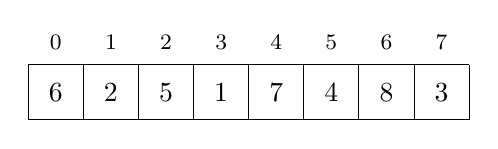
\begin{tikzpicture}[scale=0.7]
\draw (0,0) grid (8,1);
\node at (0.5,0.5) {$6$};
\node at (1.5,0.5) {$2$};
\node at (2.5,0.5) {$5$};
\node at (3.5,0.5) {$1$};
\node at (4.5,0.5) {$7$};
\node at (5.5,0.5) {$4$};
\node at (6.5,0.5) {$8$};
\node at (7.5,0.5) {$3$};

\footnotesize
\node at (0.5,1.4) {$0$};
\node at (1.5,1.4) {$1$};
\node at (2.5,1.4) {$2$};
\node at (3.5,1.4) {$3$};
\node at (4.5,1.4) {$4$};
\node at (5.5,1.4) {$5$};
\node at (6.5,1.4) {$6$};
\node at (7.5,1.4) {$7$};
\end{tikzpicture}
\end{center}
es té que la subseqüència creixent més llarga
conté 4 elements:
\begin{center}
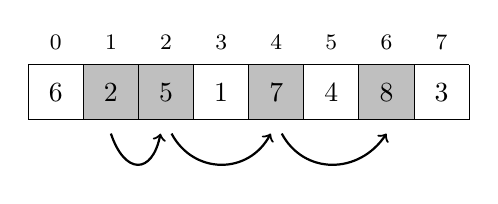
\begin{tikzpicture}[scale=0.7]
\fill[color=lightgray] (1,0) rectangle (2,1);
\fill[color=lightgray] (2,0) rectangle (3,1);
\fill[color=lightgray] (4,0) rectangle (5,1);
\fill[color=lightgray] (6,0) rectangle (7,1);
\draw (0,0) grid (8,1);
\node at (0.5,0.5) {$6$};
\node at (1.5,0.5) {$2$};
\node at (2.5,0.5) {$5$};
\node at (3.5,0.5) {$1$};
\node at (4.5,0.5) {$7$};
\node at (5.5,0.5) {$4$};
\node at (6.5,0.5) {$8$};
\node at (7.5,0.5) {$3$};

\draw[thick,->] (1.5,-0.25) .. controls (1.75,-1.00) and (2.25,-1.00) .. (2.4,-0.25);
\draw[thick,->] (2.6,-0.25) .. controls (3.0,-1.00) and (4.0,-1.00) .. (4.4,-0.25);
\draw[thick,->] (4.6,-0.25) .. controls (5.0,-1.00) and (6.0,-1.00) .. (6.5,-0.25);

\footnotesize
\node at (0.5,1.4) {$0$};
\node at (1.5,1.4) {$1$};
\node at (2.5,1.4) {$2$};
\node at (3.5,1.4) {$3$};
\node at (4.5,1.4) {$4$};
\node at (5.5,1.4) {$5$};
\node at (6.5,1.4) {$6$};
\node at (7.5,1.4) {$7$};
\end{tikzpicture}
\end{center}

Sigui $\texttt{longitud}(k)$
la longitud de la
subseqüència creixent més llarga
que acaba a la posició $k$.
Si calculèssim tots els valors de
$\texttt{longitud}(k)$ on $0 \le k \le n-1$,
descobriríem quina és la longitud de la
subseqüència creixent més llarga.
Per exemple, els valors de la funció
per al vector anterior són els següents:
\[
\begin{array}{lcl}
\texttt{longitud}(0) & = & 1 \\
\texttt{longitud}(1) & = & 1 \\
\texttt{longitud}(2) & = & 2 \\
\texttt{longitud}(3) & = & 1 \\
\texttt{longitud}(4) & = & 3 \\
\texttt{longitud}(5) & = & 2 \\
\texttt{longitud}(6) & = & 4 \\
\texttt{longitud}(7) & = & 2 \\
\end{array}
\]

Per exemple, $\texttt{longitud}(6)=4$,
perquè la subseqüència creixent més llarga
que acaba a la posició 6 consta de 4 elements.

Per calcular un valor de $\texttt{longitud}(k)$,
hauríem de trobar una posició $i<k$
per a la qual $\texttt{v}[i]<\texttt{v}[k]$
i $\texttt{longitud}(i)$ és tan gran com sigui possible.
D'aquí deduïm que
$\texttt{longitud}(k)=\texttt{longitud}(i)+1$,
perquè aquesta és una manera òptima d'afegir
$\texttt{v}[k]$ a una subseqüència.
Tanmateix, si no existeix aquesta posició $i$,
llavors $\texttt{longitud}(k)=1$,
és a dir, l'única subseqüència possible es aquella
que només conté l'element $\texttt{v}[k]$.

Podem fer servir programació dinàmica perquè tots els valors de la
funció es poden calcular a partir de valors més petits.
En el codi següent emmagatzemem els valors de la funció en
el vector
$\texttt{longitud}$.

\begin{lstlisting}
for (int k = 0; k < n; k++) {
    longitud[k] = 1;
    for (int i = 0; i < k; i++) {
        if (v[i] < v[k]) {
            longitud[k] = max(longitud[k],longitud[i]+1);
        }
    }
}
\end{lstlisting}

Aquest codi funciona en temps $O(n^2)$
perquè consta de dos bucles niats.
Tanmateix, també és possible implementar el
càlcul anterior de programació dinàmica
de manera més eficient en temps $O(n \log n)$.
Pots trobar una manera de fer-ho?

\section{Camins en una quadrícula}

El problam següent és trobar un camí
que vagi de la cantonada superior esquerra a
la cantonada inferior dreta
d'una quadrícula $n \times n$, moguent-nos únicament
cap avall i cap a la dreta.
Cada quadrat conté un nombre enter positiu,
i el camí s'ha de construir de tal manera
que la suma dels valors al llarg
el camí sigui la més gran possible.

La imatge següent mostra un camí òptim
en una quadrícula:
\begin{center}
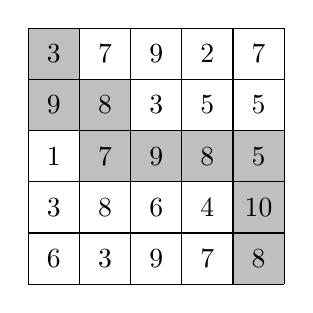
\begin{tikzpicture}[scale=.65]
  \begin{scope}
    \fill [color=lightgray] (0, 9) rectangle (1, 8);
    \fill [color=lightgray] (0, 8) rectangle (1, 7);
    \fill [color=lightgray] (1, 8) rectangle (2, 7);
    \fill [color=lightgray] (1, 7) rectangle (2, 6);
    \fill [color=lightgray] (2, 7) rectangle (3, 6);
    \fill [color=lightgray] (3, 7) rectangle (4, 6);
    \fill [color=lightgray] (4, 7) rectangle (5, 6);
    \fill [color=lightgray] (4, 6) rectangle (5, 5);
    \fill [color=lightgray] (4, 5) rectangle (5, 4);
    \draw (0, 4) grid (5, 9);
    \node at (0.5,8.5) {3};
    \node at (1.5,8.5) {7};
    \node at (2.5,8.5) {9};
    \node at (3.5,8.5) {2};
    \node at (4.5,8.5) {7};
    \node at (0.5,7.5) {9};
    \node at (1.5,7.5) {8};
    \node at (2.5,7.5) {3};
    \node at (3.5,7.5) {5};
    \node at (4.5,7.5) {5};
    \node at (0.5,6.5) {1};
    \node at (1.5,6.5) {7};
    \node at (2.5,6.5) {9};
    \node at (3.5,6.5) {8};
    \node at (4.5,6.5) {5};
    \node at (0.5,5.5) {3};
    \node at (1.5,5.5) {8};
    \node at (2.5,5.5) {6};
    \node at (3.5,5.5) {4};
    \node at (4.5,5.5) {10};
    \node at (0.5,4.5) {6};
    \node at (1.5,4.5) {3};
    \node at (2.5,4.5) {9};
    \node at (3.5,4.5) {7};
    \node at (4.5,4.5) {8};
  \end{scope}
\end{tikzpicture}
\end{center}
La suma dels valors del camí és 67,
i aquesta és la suma més gran possible per a
qualsevol camí des del
cantonada superior esquerra a la cantonada inferior dreta.

Suposem que les files i columnes del
la cuadrícula estan numerades de l'1 al $n$,
i que $\texttt{valor}[y][x]$ és el valor de la casella
$(y,x)$.
Sigui $\texttt{suma}(y,x)$ la suma màxima
de camins que van des de la cantonada superior esquerra
a la casella $(y,x)$.
Aleshores, $\texttt{suma}(n,n)$ ens diu
la suma màxima
de la cantonada superior esquerra a
la cantonada inferior dreta.
Per exemple, a la cuadrícula anterior,
$\texttt{sum}(5,5)=67$.

Les sumes màximes es poden calcular de manera recursiva
com segueix:
\[ \texttt{suma}(y,x) = \max(\texttt{suma}(y,x-1),\texttt{suma}(y-1,x))+\texttt{valor}[y][x]\]

La fórmula recursiva es basa en l'observació
que un camí que acaba a la casella $(y,x)$
ha de passar per la casella $(y,x-1)$
o la casella $(y-1,x)$:
\begin{center}
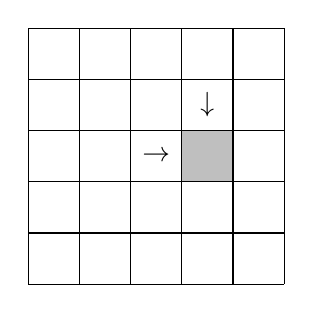
\begin{tikzpicture}[scale=.65]
  \begin{scope}
    \fill [color=lightgray] (3, 7) rectangle (4, 6);
    \draw (0, 4) grid (5, 9);
    
    \node at (2.5,6.5) {$\rightarrow$};
    \node at (3.5,7.5) {$\downarrow$};
    
  \end{scope}
\end{tikzpicture}
\end{center}

Per tant, només hem de triar la direcció que maximitzi la suma.
Si definim $\texttt{suma}(y,x)=0$
per $y=0$ o $x=0$ (els camins no poden sortir de la cuadrícula),
tenim que la fórmula recursiva també funciona quan $y=1$ o $x=1$.

Com que la funció \texttt{suma} té dos paràmetres,
el vector de la programació dinàmica també té dues dimensions.
Per exemple, podem fer servir la matriu
\begin{lstlisting}
vector<vector<int>> suma(N, vector<int>(N));
\end{lstlisting}
i calcula les sumes de la següent manera:
\begin{lstlisting}
for (int y = 1; y <= n; y++) {
    for (int x = 1; x <= n; x++) {
        suma[y][x] = max(suma[y][x-1],suma[y-1][x])+valor[y][x];
    }
}
\end{lstlisting}
La complexitat temporal de l'algorisme és $O(n^2)$.

\section{Problemes de motxilla}

\index{motxilla}

El terme \key{motxilla} (\emph{knapsack}) es refereix a problemes on
es dóna un conjunt d'objectes, i volem
buscar subconjunts amb algunes propietats.
Els problemes de motxilla sovint es poden resoldre
fent servir programació dinàmica.

En aquest apartat, ens centrem en el següent
problema: donada una llista de pesos
$[w_1,w_2,\ldots,w_n]$,
determinar totes les 
sumes que es poden construir fent servir els pesos.
Per exemple, donats els pesos
$[1,3,3,5]$, podem obtenir les següents sumes:

\begin{center}
\begin{tabular}{rrrrrrrrrrrrr}
 0 & 1 & 2 & 3 & 4 & 5 & 6 & 7 & 8 & 9 & 10 & 11 & 12 \\
\hline
 X & X & & X & X & X & X & X & X & X & & X & X \\
\end{tabular}
\end{center}

En aquest cas, totes les sumes entre $0 \ldots 12$
són possibles, excepte 2 i 10.
Per exemple, la suma 7 és possible perquè
podem seleccionar els pesos $[1,3,3]$.

Per resoldre el problema, ens centrem en els subproblemes
on només fem servir els primers $k$ pesos
per construir sumes.
Sigui $\texttt{possible}(x,k)=\textrm{true}$ si
podem construir una suma $x$
fent servir els primers $k$ pesos,
i $\texttt{possible}(x,k)=\textrm{fals}$ en cas contrari.
Els valors de la funció es poden calcular recursivament
de la següent manera:
\[ \texttt{possible}(x,k) = \texttt{possible}(x-w_k,k-1) \lor \texttt{possible}(x,k-1) \]
La fórmula es basa en el fet que podem
fer servir o no fer servir el pes $w_k$ a la suma.
Si fem servir $w_k$, la tasca restant és
trobar la suma $x-w_k$ fent servir els primers $k-1$ pesos,
i si no fem servir $w_k$,
la tasca restant és formar la suma $x$
fent servir els primers pesos $k-1$.
Els casos bàsics sónCom a casos bàsics,
\begin{equation*}
    \texttt{possible}(x,0) = \begin{cases}
               \textrm{true}    & x = 0\\
               \textrm{false}   & x \neq 0 \\
           \end{cases}
\end{equation*}
perquè si no fem servir pesos, només podem formar la suma 0.

La taula següent mostra tots els valors de la funció
per als pesos $[1,3,3,5]$ (el símbol ``X''
indica els valors reals):

\begin{center}
\begin{tabular}{r|rrrrrrrrrrrrr}
$k \backslash x$ & 0 & 1 & 2 & 3 & 4 & 5 & 6 & 7 & 8 & 9 & 10 & 11 & 12 \\
\hline
 0 & X & \\
 1 & X & X \\
 2 & X & X & & X & X \\
 3 & X & X & & X & X & & X & X \\
 4 & X & X & & X & X & X & X & X & X & X & & X & X \\
\end{tabular}
\end{center}

Després de calcular aquests valors, $\texttt{possible}(x,n)$
ens diu si podem construir la
suma $x$ fent servir \emph{tots} pesos.

Sigui $W$ la suma total dels pesos.
El codi següent es correspon a la funció recursiva anterior i troba la
solució en temps $O(nW)$.
\begin{lstlisting}
possible[0][0] = true;
for (int k = 1; k <= n; k++) {
    for (int x = 0; x <= W; x++) {
        if (x-w[k] >= 0) possible[x][k] |= possible[x-w[k]][k-1];
        possible[x][k] |= possible[x][k-1];
    }
}
\end{lstlisting}

No obstant això, en aquest cas
hi ha una millor implementació que només fa servir
un vector unidimensional $\texttt{possible}[x]$
que indica si podem construir un subconjunt amb la suma $x$.
El truc és actualitzar el vector de dreta a esquerra
per cada nou pes\footnote{N. del T.: Una solució alternativa i general consisteix
en fer servir dos vectors unidimensionals, un per la fila actual ($k$) i un per la
fila anterior ($k-1$).}:
\begin{lstlisting}
possible[0] = cert;
for (int k = 1; k <= n; k++) {
    for (int x = W; x >= 0; x--) {
        if (possible[x]) possible[x+w[k]] = true;
    }
}
\end{lstlisting}

Tingueu en compte que la idea presentada aquí es pot fer servir per
molts problemes de motxilla.
Per exemple, si ens donen objectes amb pesos i valors,
podríem determinar quin subconjunt d'objectes ens donarien valor màxim
per a cadascun dels pesos possibles.

\section{Distància d'edició}

\index{Distància d'edició}
\index{Distància de Levenshtein}

La \key{distància d'edició} o \key{distància de Levenshtein}\footnote{La distància
rep el nom de V. I. Levenshtein, que la va estudiar per la seva relació amb les
codificacions binàries \cite{lev66}.}
és el nombre mínim d'operacions d'edició
que fan falta per transformar una cadena
en una altra cadena.
Les operacions d'edició permeses són les següents:
\begin{itemize}
\item inserir un caràcter (per exemple, \texttt{ABC} $\rightarrow$ \texttt{ABCA})
\item eliminar un caràcter (per exemple, \texttt{ABC} $\rightarrow$ \texttt{AC})
\item modificar un caràcter (per exemple, \texttt{ABC} $\rightarrow$ \texttt{ADC})
\end{itemize}

Per exemple, la distància d'edició entre
\texttt{LOVE} i \texttt{MOVIE} és 2,
perquè primer podem realitzar l'operació
 \texttt{LOVE} $\rightarrow$ \texttt{MOVE}
(modificar) i després l'operació
\texttt{MOVE} $\rightarrow$ \texttt{MOVIE}
(inserir).
Aquest és el nombre més petit possible d'operacions,
perquè és evident que una sola operació no és suficient.

Suposem que se'ns dóna una cadena \texttt{x}
de longitud $n$ i una cadena \texttt{y} de longitud $m$,
i volem calcular la distància d'edició entre
\texttt{x} i \texttt{y}.
Per resoldre el problema, definim una funció
$\texttt{dist}(a,b)$ que dóna
la distància d'edició entre prefixos
$\texttt{x}[0 \ldots a]$ i $\texttt{y}[0 \ldots b]$.
Així, utilitzant aquesta funció, la distància d'edició
entre \texttt{x} i \texttt{y} és igual a $\texttt{dist}(n-1,m-1)$.

Podem calcular valors de \texttt{dist}
com segueix:
\begin{equation*}
\begin{split}
\texttt{dist}(a,b) = \min(& \texttt{dist}(a,b-1)+1, \\
                           & \texttt{dist}(a-1,b)+1, \\
                           & \texttt{dist}(a-1,b-1)+\texttt{cost}(a,b)).
\end{split}
\end{equation*}
Aquí $\texttt{cost}(a,b)=0$ si $\texttt{x}[a]=\texttt{y}[b]$,
i en cas contrari $\texttt{cost}(a,b)=1$.
La fórmula considera les següents maneres
d'editar la cadena \texttt{x}:
\begin{itemize}
\item $\texttt{dist}(a,b-1)$: inserir un caràcter al final de \texttt{x}
\item $\texttt{dist}(a-1,b)$: eliminar l'últim caràcter de \texttt{x}
\item $\texttt{dist}(a-1,b-1)$: modificar, si és necessari, l'últim caràcter
  de \texttt{x}
\end{itemize}
En els dos primers casos, fa falta una sola operació d'edició
(inserir o eliminar).
En el darrer cas, si $\texttt{x}[a]=\texttt{y}[b]$,
no fa falta gastar cap operació, pero en cas contrari
necessitem una operació d'edició (modificar).

La taula següent mostra els valors de \texttt{dist}
en el cas exemple:
\begin{center}
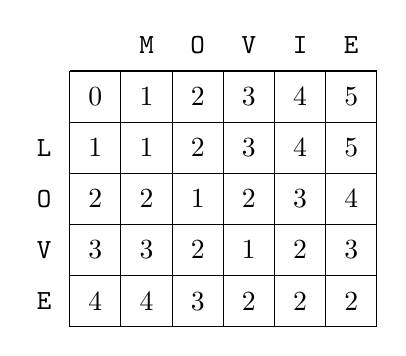
\begin{tikzpicture}[scale=.65]
  \begin{scope}
    %\fill [color=lightgray] (5, -3) rectangle (6, -4);
    \draw (1, -1) grid (7, -6);
    
    \node at (0.5,-2.5) {\texttt{L}};
    \node at (0.5,-3.5) {\texttt{O}};
    \node at (0.5,-4.5) {\texttt{V}};
    \node at (0.5,-5.5) {\texttt{E}};

    \node at (2.5,-0.5) {\texttt{M}};
    \node at (3.5,-0.5) {\texttt{O}};
    \node at (4.5,-0.5) {\texttt{V}};
    \node at (5.5,-0.5) {\texttt{I}};
    \node at (6.5,-0.5) {\texttt{E}};

    \node at (1.5,-1.5) {$0$};
    \node at (1.5,-2.5) {$1$};
    \node at (1.5,-3.5) {$2$};
    \node at (1.5,-4.5) {$3$};
    \node at (1.5,-5.5) {$4$};
    \node at (2.5,-1.5) {$1$};
    \node at (2.5,-2.5) {$1$};
    \node at (2.5,-3.5) {$2$};
    \node at (2.5,-4.5) {$3$};
    \node at (2.5,-5.5) {$4$};
    \node at (3.5,-1.5) {$2$};
    \node at (3.5,-2.5) {$2$};
    \node at (3.5,-3.5) {$1$};
    \node at (3.5,-4.5) {$2$};
    \node at (3.5,-5.5) {$3$};
    \node at (4.5,-1.5) {$3$};
    \node at (4.5,-2.5) {$3$};
    \node at (4.5,-3.5) {$2$};
    \node at (4.5,-4.5) {$1$};
    \node at (4.5,-5.5) {$2$};
    \node at (5.5,-1.5) {$4$};
    \node at (5.5,-2.5) {$4$};
    \node at (5.5,-3.5) {$3$};
    \node at (5.5,-4.5) {$2$};
    \node at (5.5,-5.5) {$2$};
    \node at (6.5,-1.5) {$5$};
    \node at (6.5,-2.5) {$5$};
    \node at (6.5,-3.5) {$4$};
    \node at (6.5,-4.5) {$3$};
    \node at (6.5,-5.5) {$2$};
  \end{scope}
\end{tikzpicture}
\end{center}

La cantonada inferior esquerra de la taula ens diu
que la distància d'edició entre
\texttt{LOVE} i \texttt{MOVIE} és 2.
La taula també mostra com construir una seqüència mínima
d'operacions d'edició. En aquest trobem el camí següent:

\begin{center}
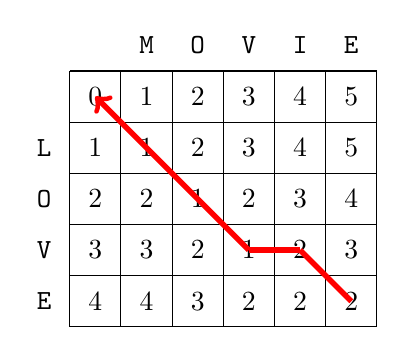
\begin{tikzpicture}[scale=.65]
  \begin{scope}
    \draw (1, -1) grid (7, -6);
    
    \node at (0.5,-2.5) {\texttt{L}};
    \node at (0.5,-3.5) {\texttt{O}};
    \node at (0.5,-4.5) {\texttt{V}};
    \node at (0.5,-5.5) {\texttt{E}};

    \node at (2.5,-0.5) {\texttt{M}};
    \node at (3.5,-0.5) {\texttt{O}};
    \node at (4.5,-0.5) {\texttt{V}};
    \node at (5.5,-0.5) {\texttt{I}};
    \node at (6.5,-0.5) {\texttt{E}};

    \node at (1.5,-1.5) {$0$};
    \node at (1.5,-2.5) {$1$};
    \node at (1.5,-3.5) {$2$};
    \node at (1.5,-4.5) {$3$};
    \node at (1.5,-5.5) {$4$};
    \node at (2.5,-1.5) {$1$};
    \node at (2.5,-2.5) {$1$};
    \node at (2.5,-3.5) {$2$};
    \node at (2.5,-4.5) {$3$};
    \node at (2.5,-5.5) {$4$};
    \node at (3.5,-1.5) {$2$};
    \node at (3.5,-2.5) {$2$};
    \node at (3.5,-3.5) {$1$};
    \node at (3.5,-4.5) {$2$};
    \node at (3.5,-5.5) {$3$};
    \node at (4.5,-1.5) {$3$};
    \node at (4.5,-2.5) {$3$};
    \node at (4.5,-3.5) {$2$};
    \node at (4.5,-4.5) {$1$};
    \node at (4.5,-5.5) {$2$};
    \node at (5.5,-1.5) {$4$};
    \node at (5.5,-2.5) {$4$};
    \node at (5.5,-3.5) {$3$};
    \node at (5.5,-4.5) {$2$};
    \node at (5.5,-5.5) {$2$};
    \node at (6.5,-1.5) {$5$};
    \node at (6.5,-2.5) {$5$};
    \node at (6.5,-3.5) {$4$};
    \node at (6.5,-4.5) {$3$};
    \node at (6.5,-5.5) {$2$};

    \path[draw=red,thick,-,line width=2pt] (6.5,-5.5) -- (5.5,-4.5);
    \path[draw=red,thick,-,line width=2pt] (5.5,-4.5) -- (4.5,-4.5);
    \path[draw=red,thick,->,line width=2pt] (4.5,-4.5) -- (1.5,-1.5);
  \end{scope}
\end{tikzpicture}
\end{center}


Els últims caràcters de \texttt{AMOR} i \texttt{MOVIE}
són iguals, de manera que la distància d'edició entre ells
és igual a la distància d'edició entre \texttt{LOV} i \texttt{MOVI}.
Podem fer servir una operació d'edició per eliminar l'últim
caràcter \texttt{I} de \texttt{MOVI}.
Per tant, la distància d'edició és un més gran que
la distància d'edició entre \texttt{LOV} i \texttt{MOV}, etc.

\section{Comptar rajoles}

De vegades, els estats d'una solució de programació dinàmica
són més complexes que les combinacions fixes de nombres.
Per exemple,
considerem el problema de calcular
el nombre de maneres diferents d'omplir
una cuadrícula $n \times m$ fent servir
fitxes de mida $1 \times 2$ i $2 \times 1$.
Una solució vàlida per a la cuadrícula $4 \times 7$ és
\begin{center}
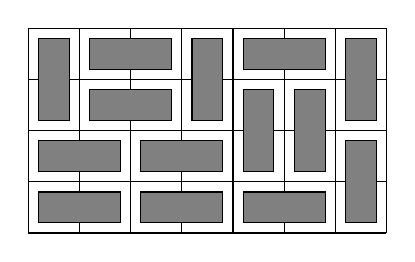
\begin{tikzpicture}[scale=.65]
    \draw (0,0) grid (7,4);
    \draw[fill=gray] (0+0.2,0+0.2) rectangle (2-0.2,1-0.2);
    \draw[fill=gray] (2+0.2,0+0.2) rectangle (4-0.2,1-0.2);
    \draw[fill=gray] (4+0.2,0+0.2) rectangle (6-0.2,1-0.2);
    \draw[fill=gray] (0+0.2,1+0.2) rectangle (2-0.2,2-0.2);
    \draw[fill=gray] (2+0.2,1+0.2) rectangle (4-0.2,2-0.2);
    \draw[fill=gray] (1+0.2,2+0.2) rectangle (3-0.2,3-0.2);
    \draw[fill=gray] (1+0.2,3+0.2) rectangle (3-0.2,4-0.2);
    \draw[fill=gray] (4+0.2,3+0.2) rectangle (6-0.2,4-0.2);

    \draw[fill=gray] (0+0.2,2+0.2) rectangle (1-0.2,4-0.2);
    \draw[fill=gray] (3+0.2,2+0.2) rectangle (4-0.2,4-0.2);
    \draw[fill=gray] (6+0.2,2+0.2) rectangle (7-0.2,4-0.2);
    \draw[fill=gray] (4+0.2,1+0.2) rectangle (5-0.2,3-0.2);
    \draw[fill=gray] (5+0.2,1+0.2) rectangle (6-0.2,3-0.2);
    \draw[fill=gray] (6+0.2,0+0.2) rectangle (7-0.2,2-0.2);

\end{tikzpicture}
\end{center}
i el nombre total de solucions és 781.

El problema es pot resoldre amb programació dinàmica
si passem per la cuadrícula fila per fila.
Cada fila d'una solució es pot representar com una
cadena que conté $m$ caràcters del conjunt
$\{\sqcap, \sqcup, \sqsubset, \sqsupset \}$.
Per exemple, la solució anterior consta de quatre files
que es corresponen amb les següents cadenes:
\begin{itemize}
\item
$\sqcap \sqsubset \sqsupset \sqcap \sqsubset \sqsupset \sqcap$
\item
$\sqcup \sqsubset \sqsupset \sqcup \sqcap \sqcap \sqcup$
\item
$\sqsubset \sqsupset \sqsubset \sqsupset \sqcup \sqcup \sqcap$
\item
$\sqsubset \sqsupset \sqsubset \sqsupset \sqsubset \sqsupset \sqcup$
\end{itemize}

Sigui $\texttt{count}(k,x)$ el nombre de maneres de construir
una solució per a les files $1 \ldots k$
de la graella de manera que la cadena $x$ correspon a la fila $k$.
Aquí és possible utilitzar la programació dinàmica,
perquè l'estat d'una fila està restringit
només per l'estat de la fila anterior.

Una solució és vàlida si la fila $1$ no conté
el caràcter $\sqcup$,
la fila $n$ no conté el caràcter $\sqcap$,
i totes les files consecutives són \emph{compatibles}.
Per exemple, les files
$\sqcup \sqsubset \sqsupset \sqcup \sqcap \sqcap \sqcup$ i
$\sqsubset \sqsupset \sqsubset \sqsupset \sqcup \sqcup \sqcap$
són compatibles, mentre que les files
$\sqcap \sqsubset \sqsupset \sqcap \sqsubset \sqsupset \sqcap$ i
$\sqsubset \sqsupset \sqsubset \sqsupset \sqsubset \sqsupset \sqcup$
no són compatibles.

Com que una fila consta de $m$ caràcters i n'hi ha
quatre opcions per a cada caràcter, el nombre de files diferents
és com a màxim $4^m$.
Per tant, la complexitat temporal de la solució és
$O(n 4^{2m})$ perquè podem passar pels
$O(4^m)$ estats possibles de cada fila
i, per a cada estat, hi ha $O(4^m)$
estats possibles de la fila anterior.
A la pràctica, és una bona idea girar la cuadrícula
per a que el costat més curt tingui longitud $m$,
donat que el factor $4^{2m}$ domina la complexitat temporal.

És possible millorar la solució amb una
representació més compacta de les files.
Resulta que n'hi ha prou amb saber quines
de les columnes de la fila anterior contenen el quadrat superior
d'una rajola vertical.
Així, podem representar una fila utilitzant només caràcters
$\sqcap$ i $\Box$, on $\Box$ és una combinació
de caràcers
$\sqcup$, $\sqsubset$ i $\sqsupset$.
Fent servir aquesta representació, només n'hi ha
$2^m$ files diferents, i la complexitat temporal és
$O(n 2^{2m})$.

Com a nota final, també hi ha una fórmula directa sorprenent
per calcular el nombre de rajoles\footnote{Sorprenentment,
aquesta fórmula va ser descoberta l'any 1961 per dos equips de recerca \cite{kas61,tem61}
que funcionaven de manera independent.}:
\[ \prod_{a=1}^{\lceil n/2 \rceil} \prod_{b=1}^{\lceil m/2 \rceil} 4 \cdot (\cos^2 \frac{\pi a }{n + 1} + \cos^2 \frac{\pi b}{m+1})\]
Aquesta fórmula és molt eficient, perquè calcula
el nombre de mosaics en $O(nm)$ temps,
però com que la resposta és un producte de nombres reals,
fer servir la fórmula requereix 
emmagatzemar els resultats intermedis amb precisió.
